\documentclass{article}
\usepackage{graphicx}
\usepackage[utf8]{inputenc}
\usepackage[vmargin=3.25cm,hmargin=3.25cm]{geometry}
\usepackage{hyperref}

\title{Finding Breakpoints of Viral Genomes using recan}
\author{Abinu Ajithan Jyothini}
\date{August 6th 2020}
\begin{document}

\maketitle
\section{Introduction}
In many different group of viruses recombination of genetic material is an important evolutionary process that generates much of genetic diversity.The patterns of recombination evident within the genomes of viruses can reveal lots of detail about their evolution and biology.Recombination is responsible for the evolution of viruses in response to selective forces present in a host environment \cite{perez2015recombination}. A better understanding of recombination events taking place in the genomes of viruses are useful for gaining in-sites about the biology of the viruses.The patterns of sequence exchange between viruses in different species can reveal otherwise undetectable ecological links between some species and barriers between others.\cite{martin2015rdp4}. The breakpoints of genomes can reveal details about mechanistic and biochemical processes regarding the recombination process.\cite{martin2015rdp4}.This project makes use of the python package 'recan'\cite{babin2020recan}(recombination analyzer) for constructing genetic distance plots and exploring them.Also, we make use of bio-python\cite{chapman2000biopython} package for plotting fasta sequences.
\section{Methods:}
\subsection{recan Python Package:}
recan is a python package developed for the recombination analysis and it provides a mean for constructing genetic distance plots and exploring them interactively.recan is based on python packages like Biopython, Pandas, Matplotlib, and Plotly libraries.recan requires the input to be in the form of alligned fasta sequence.There are options for changing the window size,adjusting the sequence of interest(for example; sequence where the breakpoints occurs), changing the method of distance calculations etc.

\subsection{Input Data:}
The fasta sequence of viral genomes can be obtained from any of the protein data banks. RCSB protein data bank \cite{rose2016rcsb}(https://www.rcsb.org/) is most popular among bioinformatic  scientists.  We can directly obtain the fasta sequence of the genome from RCSB.Since the recan only takes aligned fasta format of the genome, the fasta sequence downloaded from the RCSB protein data bank needs to be alligned.This can be achieved by using NCBI Multiple SEquence Allignment Viewer(https://www.ncbi.nlm.nih.gov/projects/msaviewer/).In this project, i chose lumky skin disease virus's genome \cite{sprygin2018epidemiological} for finding out the breakpoints. I have also used the genome sequence of BCRA1 genes, which are the genes that produce tumor suppressor proteins, for demonstrating the visualization of the fasta sequence.

\section{Results and Discussion:}
\subsection{Breakpoints:}
In genetics, the rearrangement of chromosomes is called mutation.It is an abnormality in the chromosome involving a change in the native chromosome  \cite{zhao2012genome}.Theses changes may involve  several events such as, duplication, inversion, deletion and translocation.These events are usually caused by a breakage in the helices of DNA and rejoining of the broken ends to form a new gene,different from the gene order of the chromosomes before they were broken \cite{griffiths2002modern}.Some regions of chromosomes are more susceptible for rearrangements than others and thus are sources of genetic diseases and cancer.The Figure\ref{Figure:1} shows the breakpoints of lumky skin disease viral genome.

\begin{figure}
    \centering
    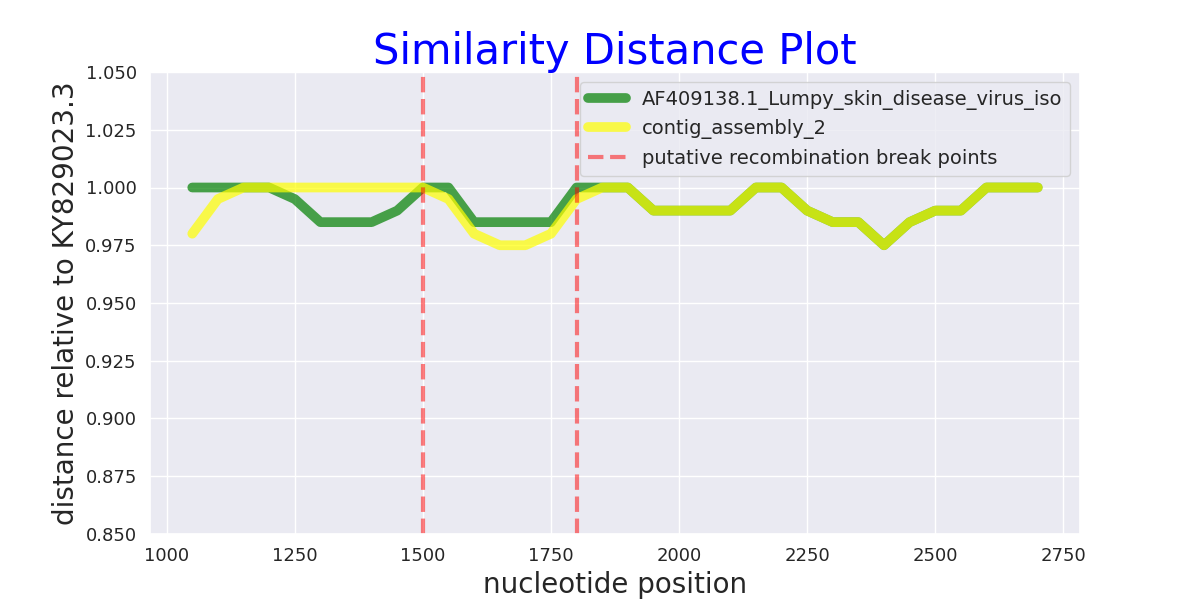
\includegraphics[height=8cm]{distance_plot}
    \caption{Distance Plot}
    \label{Figure:1}
\end{figure}
















\begin{figure}
    \centering
    \includegraphics[width=0.9\textwidth]{}
    \caption{Caption}
    \label{ternary}
\end{figure}

\begin{figure}
    \centering
    \includegraphics[width=0.9\textwidth]{}
    \caption{Caption}
    \label{ternary}
\end{figure}



\bibliography{rsc.bib} 
\bibliographystyle{unsrt}
\end{document}
